\documentclass[11pt]{article}
\usepackage{amsmath, amssymb, amsthm}
\usepackage{fullpage}
\usepackage{tikz}
\usetikzlibrary{shapes.geometric}
\usetikzlibrary{arrows}
\usepackage{amsmath}
\usepackage{hyperref}

\newcounter{excounter}
\setcounter{excounter}{1}
\newcommand\question[2]{\vskip 1em  \noindent\textbf{\arabic{excounter}\addtocounter{excounter}{1}:} (\emph{#1}) \newline \noindent#2}
\newcommand\hint[1]{ \newline \noindent\textit{Hint: #1}}
\newcommand\solution[1]{\vskip 0.5em \noindent\textbf{Solution:}\par\noindent#1}




\begin{document}
\large

{\bf MATH-566 \hspace{1cm} HW 08}
\vskip 1em
Due \textbf{Nov 9} before class (regularly). Just bring it before the class and it will be collected there.


Consider the following network $M$ with costs and capacities depicted on edges
and boundary in vertices.

\begin{center}
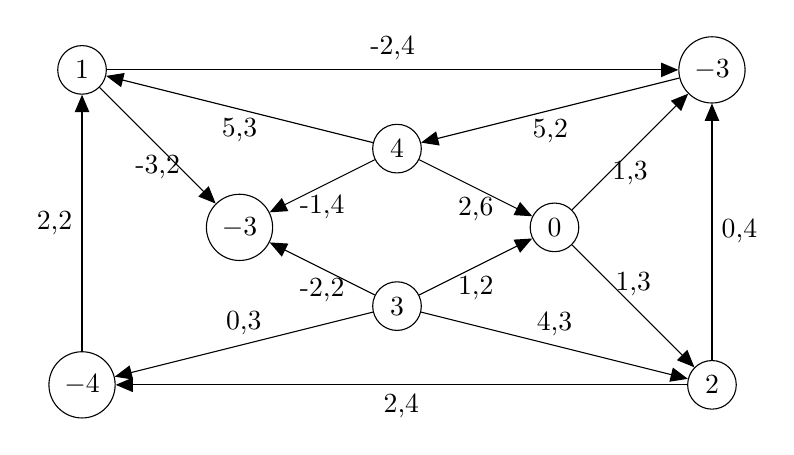
\begin{tikzpicture}[xscale=2]
\draw 
(0,0) node[draw,circle](x){$-4$}
(4,0) node[draw,circle](y){$2$}
(0,4) node[draw,circle](z){$1$}
(4,4) node[draw,circle](w){$-3$}
(2,1) node[draw,circle](a){$3$}
(1,2) node[draw,circle](b){$-3$}
(2,3) node[draw,circle](c){$4$}
(3,2) node[draw,circle](d){$0$}
;
\foreach \x/\y/\l in {y/x/{2,4} , z/b/{-3,2}, d/w/{1,3},c/b/{-1,4},c/d/{2,6},a/b/{-2,2},a/d/{1,2},
c/z/{5,3}, w/c/{5,2}  }{
\draw[-triangle 45](\x)--node[below]{\l}(\y);
}
\foreach \x/\y/\l in {z/w/{-2,4}, a/x/{0,3}, a/y/{4,3}, d/y/{1,3} }{
\draw[-triangle 45](\x)--node[above]{\l}(\y);
}
\foreach \x/\y/\l in {x/z/{2,2} }{
\draw[-triangle 45](\x)--node[left]{\l}(\y);
}
\foreach \x/\y/\l in {y/w/{0,4} }{
\draw[-triangle 45](\x)--node[right]{\l}(\y);
}
\end{tikzpicture}
\end{center}


\question{Try Min Cost Flow algorithm}{
Consider the following $b$-flow $f$ in $M$.


\begin{center}
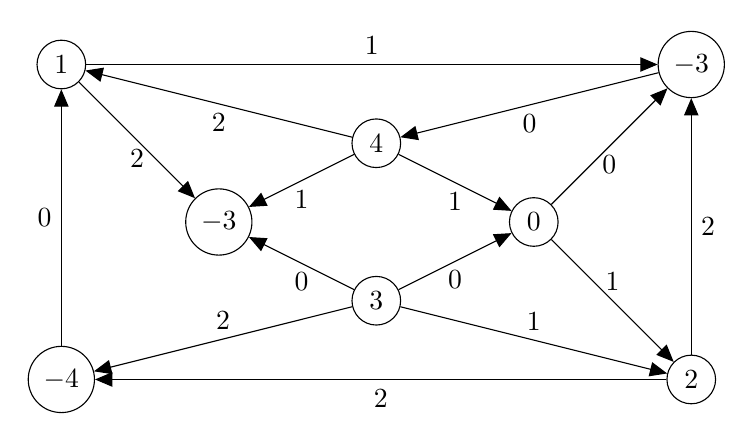
\begin{tikzpicture}[xscale=2]
\draw 
(0,0) node[draw,circle](x){$-4$}
(4,0) node[draw,circle](y){$2$}
(0,4) node[draw,circle](z){$1$}
(4,4) node[draw,circle](w){$-3$}
(2,1) node[draw,circle](a){$3$}
(1,2) node[draw,circle](b){$-3$}
(2,3) node[draw,circle](c){$4$}
(3,2) node[draw,circle](d){$0$}
;
\foreach \x/\y/\l in {y/x/{2} , z/b/{2}, d/w/{0},c/b/{1},c/d/{1},a/b/{0},a/d/{0},
c/z/{2}, w/c/{0}  }{
\draw[-triangle 45](\x)--node[below]{\l}(\y);
}
\foreach \x/\y/\l in {z/w/{1}, a/x/{2}, a/y/{1}, d/y/{1} }{
\draw[-triangle 45](\x)--node[above]{\l}(\y);
}
\foreach \x/\y/\l in {x/z/{0} }{
\draw[-triangle 45](\x)--node[left]{\l}(\y);
}
\foreach \x/\y/\l in {y/w/{2} }{
\draw[-triangle 45](\x)--node[right]{\l}(\y);
}
\end{tikzpicture}
\end{center}

Compute the cost of $f$.

Start computing the minimum cost $b$-flow by finding a sequence of augmenting cycles starting from $f$.
(No need to use minimum mean cycles, do two augmentations. No need to solve it to optimality.)

You may use  the following template to create residual graphs for finding the cycle.
\begin{center}
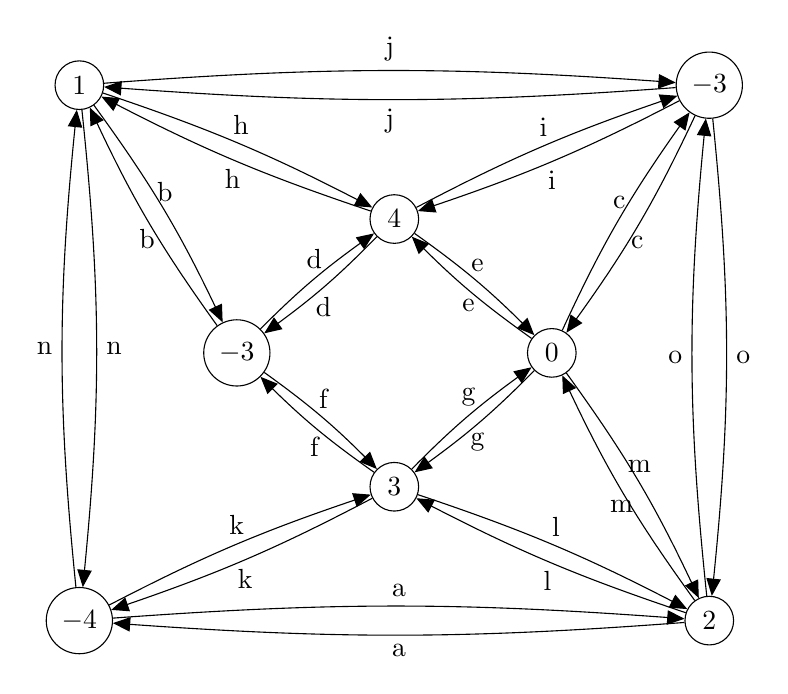
\begin{tikzpicture}[xscale=2,yscale=1.7]
\draw 
(0,0) node[draw,circle](x){$-4$}
(4,0) node[draw,circle](y){$2$}
(0,4) node[draw,circle](z){$1$}
(4,4) node[draw,circle](w){$-3$}
(2,1) node[draw,circle](a){$3$}
(1,2) node[draw,circle](b){$-3$}
(2,3) node[draw,circle](c){$4$}
(3,2) node[draw,circle](d){$0$}
;
%%% Labels below
\foreach \x/\y/\l in {y/x/{a} , b/z/{b}, w/d/{c},c/b/{d},d/c/{e},a/b/{f},d/a/{g},
c/z/{h}, w/c/{i}, w/z/{j}, a/x/{k}, y/a/{l}, y/d/{m}  }{
\draw[-triangle 45](\x) to[bend left=5] node[below]{\l}(\y);
}
%%% Labels above
\foreach \x/\y/\l in {y/x/{a} , b/z/{b}, w/d/{c},c/b/{d},d/c/{e},a/b/{f},d/a/{g},
c/z/{h}, w/c/{i}, w/z/{j}, a/x/{k}, y/a/{l}, y/d/{m}  }{
\draw[-triangle 45](\y) to[bend left=5] node[above]{\l}(\x);
}
%%% Labels left
\foreach \x/\y/\l in {x/z/{n}, y/w/{o} }{
\draw[-triangle 45](\x) to[bend left=5]  node[left]{\l}(\y);
}
%%% Labels right
\foreach \x/\y/\l in {x/z/{n}, y/w/{o} }{
\draw[-triangle 45](\y) to[bend left=5]  node[right]{\l}(\x);
}

\end{tikzpicture}
\end{center}
}





\question{Min Cost Flow as Linear Program}{
Solve minimum cost $b$-flow for $M$ using linear programming.
That is, formulate the problem using linear programming and solve it
using Sage or APMonitor. Then draw the resulting network.
}



\question{Max Flow $\subset$ Min Cost Flow}{
Show that the Maximum Flow Problem can be regarded as a special case of the Minimum Cost Flow problem.
That is, for an instance of Maximum Flow Problem find a reformulation to Minimum Cost Flow problem whose
solution can be interpreted as a solution to Maximum Flow Problem.
That is, find \emph{simple} algorithm that is solving Maximum Flow Problem and using Minimum Cost Flow as
a black box subroutine once.
}



\end{document}









